\chapter{Implementation \& Evaluation}
\label{ch:impl_eval}
\section{Baseline with MCTS}
In order to develop a non-trivial strategy for an enemy playing the game(s) developed in chapter \ref{ch:modelling}, we'll use  the MCTS algorithm described in section \ref{sec:intro_mcts}.
While we could use MCTS in stead of MARL algorithms, MCTS does have some properties that make it unsuitable for our purposes. Firstly, it uses the complete state information of the game. Secondly, while it generally outperforms simpler algorithms like minimax, it still doesn't scale to more realistic situations. Furthermore, since MCTS works on turn-based games, the game from chapter \ref{ch:modelling} is adapted to accommodate executing actions in sequence for the two players.\\

However, it does allow us to develop strategies for two opposing players form the ground up. Thus using MCTS at this phase has two purposes:
\begin{enumerate}
    \item Analyzing the performance of the algorithm
    \item Obtaining a baseline opponent policy against which the MARL algorithms can be evaluated.
\end{enumerate}

% ----------------------------------------------------------------------------------------

%\section{Innateness vs. Learned}
%\textbf{Discuss advantages / disadvantages of innate knowledge (e.g. no aim/fire when not in range $\rightarrow$ might be valid initial knowledge, while simple strategies might not)} 

\section{First Model}
\subsection{Independent RL}
\label{sec:iql_applied}
This section discusses the application of Independent Deep Policy Gradients (section \ref{sec:intro_deep_indep_rl}) to the simple battlefield model described in section \ref{sec:first_model}. Two agents were trained with DPG (in casu the simple REINFORCE algorithm) on a 7-by-7 board against two opposing players who made random moves. The maximum range for all players was $5$ steps, so agents have to learn to approach other agents before firing.\\

A comment on the random opponents: agents that make random moves are indeed simple to beat; the final goal however is to work in an iterative fashion: 
\begin{enumerate}
    \item Train two agents against two random agents.
    \item Train two new agents against these two already trained agents until they can consistently beat them.
    \item Continue in this way until no more progress is made.
\end{enumerate}
The figures below summarize the results of the first point.\\
% Nov13_10-05-55_ideapad-pg smoothing 0.95
% Add (insert): run 171

The training of both agents was run for 3000 episodes, generated by sampling actions from the policy $\pi_i(a_t|s_t)$ and interacting with the environment. Figures \ref{fig:exp1_loss0} and \ref{fig:exp1_loss1} show how the mean gradient $G_t \, \nabla_{\bm{\theta}} \ln \pi(A_t|S_t,\bm{\theta})$ evolves in the time (see the REINFORCE algorithm \ref{algo:reinforce}) for both agents. This "loss" gives an indication of the evolution of the network parameters. Notice how both graphs evolve to zero, meaning that the agents have reached their goal and are no longer learning.\\
\begin{figure}
\centering
\begin{minipage}{.5\textwidth}
  \centering
  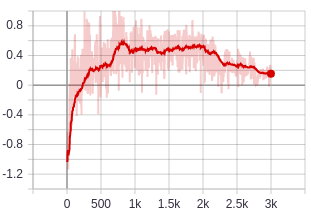
\includegraphics[width=7cm]{images/experiment1/loss_T0.png}
  \captionof{figure}{Gradient estimate for agent $0$}
  \label{fig:exp1_loss0}
\end{minipage}%
\begin{minipage}{.5\textwidth}
  \centering
  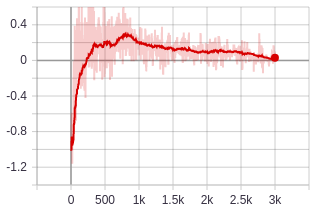
\includegraphics[width=7cm]{images/experiment1/loss_T1.png}
  \captionof{figure}{Gradient estimate for agent $1$}
  \label{fig:exp1_loss1}
\end{minipage}
\end{figure}

Figure \ref{fig:exp1_length} shows the average duration of an episode. Notice that initially, when the agent's policy network has random weights and he effectively functions as a random agent, the episodes take a long time because nobody is taking any directed actions. Once the agent's learns from experience, his behavior becomes more directive and the episode duration decreases rapidly. Figure \ref{fig:exp1_reward} shows the average reward per episode for the agents. Initially, the agents lose more often than they win; the win rate increases rapidly and finally the agents win always all the time. This curve is called the \emph{learning curve} and will be the standard way to evaluate the performance of a MARL algorithm.\\

\begin{figure}
\centering
\begin{minipage}{.5\textwidth}
  \centering
  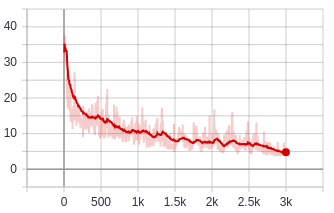
\includegraphics[width=7cm]{images/experiment1/mean_length.png}
  \captionof{figure}{Mean episode length}
  \label{fig:exp1_length}
\end{minipage}%
\begin{minipage}{.5\textwidth}
  \centering
  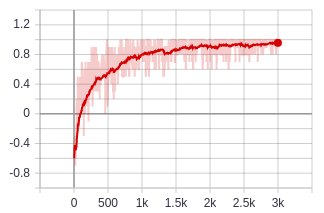
\includegraphics[width=7cm]{images/experiment1/mean_reward.png}
  \captionof{figure}{Mean reward for agents of the first player}
  \label{fig:exp1_reward}
\end{minipage}
\end{figure}
In this simple scenario, the agents have learned to (in this order):
\begin{enumerate}
    \item Aim at the opposing agents (resp. $0 \rightarrow 2$ and $1 \rightarrow 3$).
    \item Come closer until the opposing agent is in range.
    \item Fire once the opposing agent is in range.
\end{enumerate}
\textbf{To mention}: use of optimizer (\emph{ADAM}) and learning rate.\\

The next evolution is to represent the agent as a recurrent neural network as explained in section \ref{sec:deep_pg}. The input of the network are the two major components of the state vector $\bm{s_t}$:
\begin{enumerate}
    \item The game board, namely the actual position of the agent relative to the board and each other, and
    \item Additional information about the agents (are they alive? What is the ammo level?)
\end{enumerate}
The board information is well suited to serve as input of a convolutional layer, since it contains spatial information. The additional information on the other hand will be fed to a fully-connected neural network layer. The result of both these layers is then combined and serves as the input for the a fully-connected layer. The output of this layer is then fed to a GRU. The neural net will have two heads, as explained in section \ref{sec:deep_pg}, and can thus be used in an actor-critic algorithm. An overview of the agent's neural network is shown in figure \ref{fig:agent_net}.
\begin{figure}[htp]
    \centering
    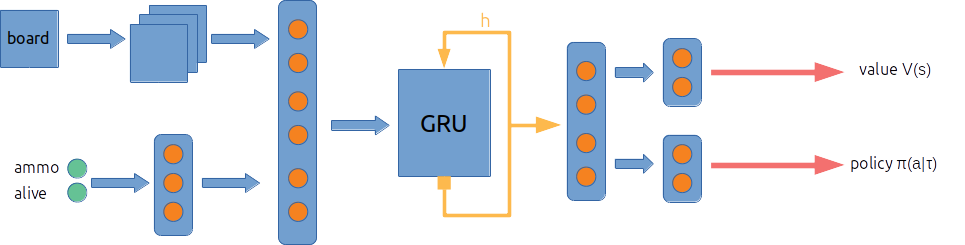
\includegraphics[width=16cm]{images/agent_net.png}
    \caption{Actor-critic agent with recurrent net}
    \label{fig:agent_net}
\end{figure}

While this modification might result in a theoretical improvement, this is not the case in practice. Figure \ref{fig:newplot194_195} shows the learning curve for agents with non-recurrent (blue) and recurrent neural nets (green). While both learn a winning strategy, it is not feasible to say one approach is better than the other. \textbf{TODO}: improve this (correct or explain).

% comparison 194-195
\begin{figure}[htp]
    \centering
    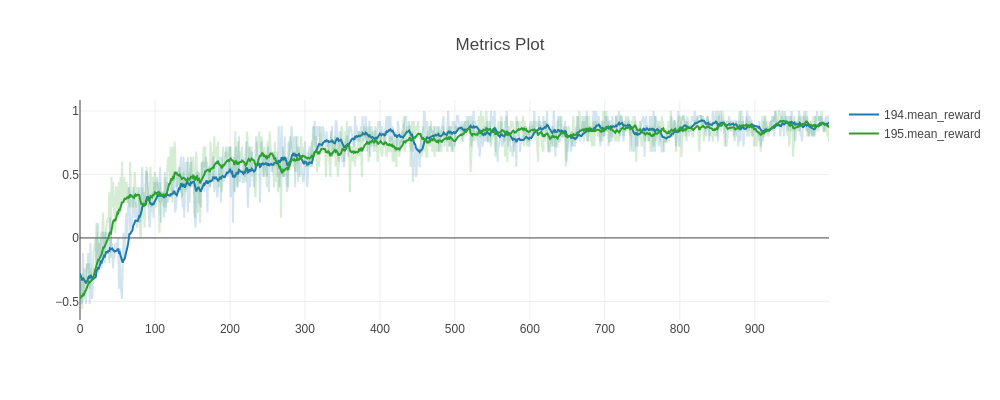
\includegraphics[width=16cm]{images/experiment2/newplot194_195.png}
    \caption{Actor-critic agent with recurrent net}
    \label{fig:newplot194_195}
\end{figure}

\subsection{COMA}
\subsection{QMIX}

\section{Second Model}
\subsection{Independent RL}
\subsection{COMA}
\subsection{QMIX}